\chapter{Архитектура Трансформер и модель BERT}\label{trbert}

\section{Архитектура Трансформер}

В предыдущих разделах были изложены предыдущие этапы развития нейросетевых моделей. На момент проведения описываемых в данной диссертационной работе научных исследований, ключевую роль в обработке текста играли модели на базе архитектуры Трансформер. В связи с этим в данном разделе будет подробно описана данная нейросетевая архитектура, а в следующем разделе - многозадачные нейросетевые модели на основе данной архитектуры, являющиеся предметом данной диссертационной работы. 

Архитектура Трансформер была разработана авторами статьи "Attention is All You Need" \cite{vaswani_2017}, выпущенной в 2017 году. Составляющие данной архитектуры - это полносвязные слои и механизм внимания(Attention). Механизм внимания был предложен авторами статьи , чтобы лучше передавать информацию из энкодера декодеру в seq2seq моделях: состояние декодировщика обновляется на основе информации от кодировщика.  

\textbf{Self-attention}(самовнимание) - это механизм внимания, примененный к самой же входной последовательности для ее обновления, Данное понятие было предложено в работе «A structured self-attentive sentence embedding» \cite{lin_2017}. Там оно применялось для векторизации предложения, что было необходимо для решения задач классификации текста. В архитектуре Трансформер модуль Attention используется как Self-attention.  

Механизм внимания работает на основе 3 матриц:  Q (Query, запрос), K(Key, ключ), V(Value, значение). 
Получая на вход последовательность токенов длины $N_{queries}$, модель до применения Self-attention векторизует каждый из данных токенов, ставя каждому токену в соответствие вектор длины $D$. Получив тем самым представление для каждого предложения - Query размерности $N_{queries}*D$, механизм также использует Key той же размерности $N_{keys}*D$ ($N_{keys}= N_{queries})$ и Value размерности $N_{keys}*D_{v}$ для формирования взвешенного скалярного произведения в соответствии со следующей формулой:

\begin{equation}
\color{black} Attention(Q, K, V) = softmax(QK^{T}V)/sqrt(D)
\label{eq:ref}
\end{equation}
\begin{figure}[ht]
  \centerfloat{
    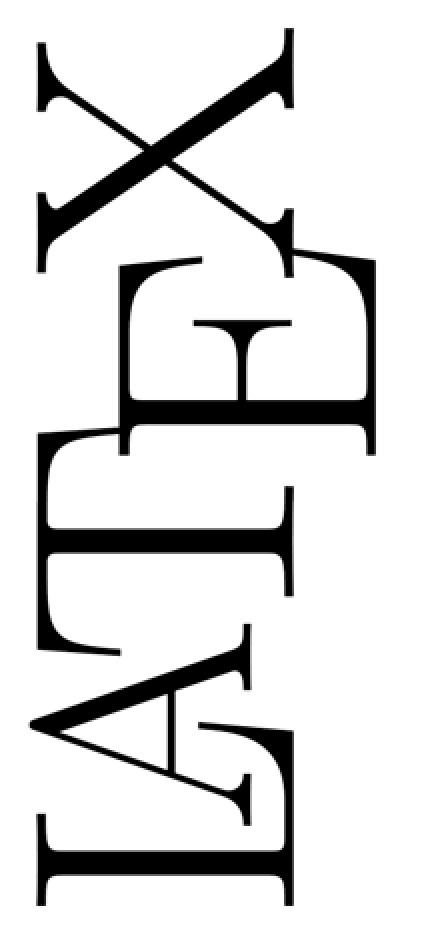
\includegraphics[scale=0.27]{latex}
  }
  \caption{Механизм Attention.}\label{fig:Transformer1-Attention}
\end{figure}


Внимание делится на $\sqrt{D}$, чтобы избежать затухания градиентов, подробнее описанного в \cite{hochreiter_1998}. 
Механизм внимания может широко применяться в задачах, которые требуют использования части входных данных - парсинг синтаксических зависимостей, понимание текста и пр. Механизм внимания особенно примечателен своей интерпретируемостью, так как он помогает понять, на какие части текста смотрит модель, за счет своих весовых коэффициентов.
Чтобы увеличить число вариаций, которыми представляются поступающие на вход токены, данный модуль в архитектуре Трансформер применяется h раз параллельно, после чего результаты этих применений конкатенируются следующим образом
\begin{equation}
\color{black} MultiHeadAttention(Q, K, V) = Concat(head_{1},... head_{h})W^{O} \label{tr:0}
\end{equation}
где
\begin{equation}
\color{black} head_{i} = Attention(QW_{i}^{Q},KW_{i}^{K},VW_{i}^{V}) \label{tr:1}
\end{equation},
где $W_{i}^{Q}$ - матрица линейного преобразования для запросов, имеющая размерность $D*D$, $W_{i}^{K}$ - матрица линейного преобразования для ключей, имеющая размерность $D*D$, $W_{i}^{V}$ - матрица линейного преобразования для значений, имеющая размерность $D*D_{v}$

Подобное применение self-attention называется "Multi-head self-attention" (многоголовое самовнимание). Оно проиллюстрировано на рисунке ниже.



\begin{figure}[ht]
  \centerfloat{
    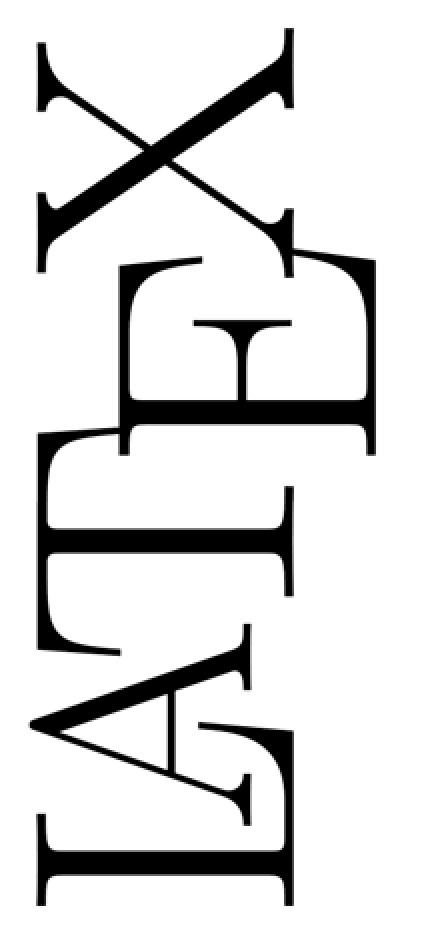
\includegraphics[scale=0.27]{latex}
  }
  \caption{Многоголовое самовнимание.}\label{fig:Transformer2-MultiHeadSelfAttention}
\end{figure}


Число голов h выбирается авторами модели вручную. Как правило, чем больше слоев у модели Трансформер, тем больше голов. 
В архитектуре Трансформер механизм внимания используется, чтобы передавать информацию с предыдущего слоя на следующий. Механизм внимания применяется к самой входной последовательности. Отличие передачи информации в двуслойной рекуррентной сети от передачи информации в Трансформере приведено на рисунке ниже. 


\begin{figure}[ht]
  \centerfloat{
    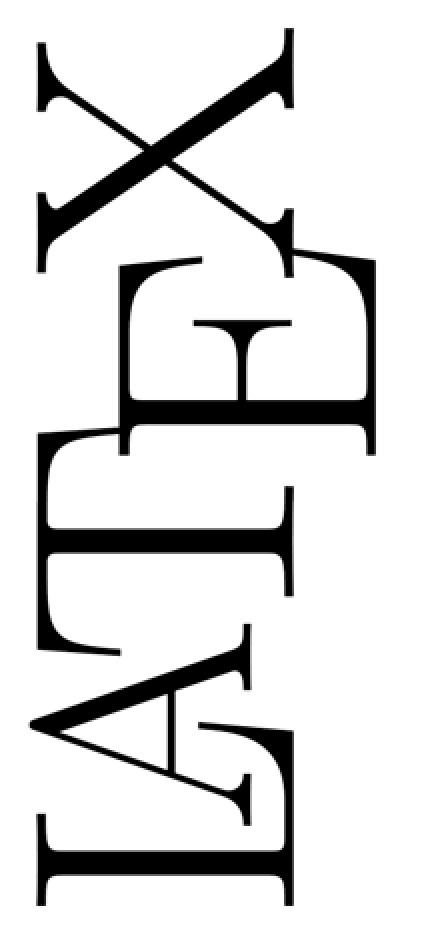
\includegraphics[scale=0.27]{latex}
  }
  \caption{Передача информации в рекуррентной и Трансформер сетях.}\label{fig:Transformer3-CompareToRNN}
\end{figure}


В архитектуру Трансформер входят повторяющиеся полносвязные слои и механизмы внимания. Они образуют Трансформер слои, из которых состоят кодировщик и декодировщик. Кодировщик состоит из некого числа N повторящихся слоев типа "многоголовое само-внимание + полносвязный слой", где полносвязный слой применяется к каждому элементу последовательности независимо. В кодировщике также используются остаточные (residual) связи вокруг этих слоев, описанные в \cite{he_2016}, и нормализации слоя, описанная в \cite{ba_2016}.
Декодировщик состоит из N повторяющихся слоев типа "многоголовое само-внимание + внимание на последний слой кодировщика + полносвязный слой". 
 Подробнее модули кодировщика и декодировщика изображены на рисунке ниже. 

\begin{figure}[ht]
  \centerfloat{
    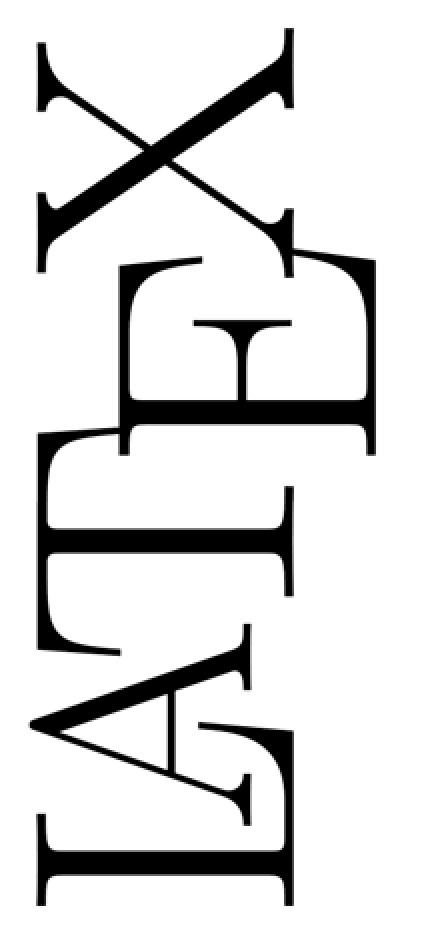
\includegraphics[scale=0.27]{latex}
  }
  \caption{Модули кодировщика и декодировщика в архитектуре Трансформер.}\label{fig:Transformer4-EncoderDecoder}
\end{figure}


 Заметим, что, поскольку декодировщик предсказывает следующее слово по предыдущим, он не может видеть информацию о будущих словах во время обучения. Поэтому в декодировщике используется маскированное само-внимание(masked self-attention). Модуль MASK “маскирует” следующие слова.
Заметим, что порядок элементов входной последовательности в оригинальной архитектуре Трансформер никак не используется, так как каждая из операций в Трансформер слое, что в кодировщике, что в декодировщике, происходит независимо для разных элементов последовательности. 

В статьях \cite{devlin_2018,gehring_2017,vaswani_2017} предложен следующий способ добавления информации о положении данного токена во входной последовательности - векторные представления позиций (position embeddings). Данные векторные представления суммируются со входными векторными представлениями. Они могут задаваться аналитически, а могут обучаться вместе с параметрами всей модели.
Архитектура Трансформер получила большое развитие за последние годы. Так, в репозитории компании HuggingFace \cite{na_website_ndaa} находится более 16 тысяч моделей, имеющих данную архитектуру, в том числе дообученных на конкретную задачу. 

Самой популярной моделью на основе архитектуры Трансформер является модель BERT, которая широко использовалась в дальнейшей работе. Эта модель описана подробнее в следующем разделе. 

\section{Языковые модели BERT}

BERT(Bidirectional Encoder Representations from Transformer) \cite{devlin_2018} - основанные на архитектуре Tрансформер модели для обработки естественного текста, предобученные одноимённым методом на задачах предсказания токена по контексту и определения того, могут ли данные 2 предложения следовать одно за другим. BERT - это универсальная архитектура. На базе BERT могут работать различные модели NLP - модели классификации одного предложения, классификации пары предложений, , регрессии, выбора из вариантов, вопросно-ответные и так далее. Модели на основе BERT значительно превзошли модели предыдущего поколения для обработки естественного языка. 
Данный метод имеет следующие ключевые особенности:
\begin{itemize}
\item[*] Обработка всей последовательности одновременно. По определению авторов, это двунаправленная(bidirectional) обработка. Отличие данного способа обработки от применяемого в двунаправленных рекуррентных сетях заключается в следующем: в двунаправленных сетях обработка входных данных производится по одному токену слева направо и справа налево, последовательно. А в нейронных сетях, имеющих архитектуру Трансформер, включая BERT, обработка каждого токена производится параллельно, при этом каждый токен имеет доступ при помощи механизма внимания ко всем остальным токенам. 
\item[*] Предобучение без учителя,или точнее, с самообучением (self supervised learning). Предобучение модели BERT требует большого объёма неразмеченных текстов, разметку для которых при этом можно получить из самих этих текстов, используя уже имеющуюся в них информацию.
\end{itemize}
Обучение модели BERT делится на 2 стадии: предобучение(pretraining) на большом объеме неразмеченных текстов и дообучение(finetuning) на относительно небольшом объёме данных, специфических для каждой конкретной задачи. 

Предобучение производится на две задачи. Первой из двух задач является Маскированное языковое моделирование (Masked Language Modeling, MLM). В данной задаче некоторые входящие токены последовательности маскируются, заменяясь на служебный токен [MASK]. Модель BERT учится предсказывать маскированные токены. Так как токен [MASK] не используется при дообучении (fine-tuning) модели, то замена производится следующим образом: каждый из 15\% случайно выбранных токенов с вероятностью 80\% заменяется на токен [MASK] (I feel very well заменяется, например, на I feel [MASK] well), с вероятностью 10\% заменяется на другой токен (I feel very well - >I feel blue well), с вероятностью 10\% не изменяется (I feel very well - >I feel very well). Эти 15\% токенов предсказываются на основе векторных представлений на финальном слое модели BERT. В качестве функции потерь используется кросс-энтропия, в качестве финальной функции активации Softmax. 

Помимо описанной выше задачи, модель BERT также необходимо научить работать с текстом не только на уровне одного предложения, но и на уровне нескольких предложений. Для этого модель BERT также учится предсказывать, может ли одно предложение встретиться после другого или нет. Данная задача называется Next Sentence Prediction (NSP). В качестве положительных примеров в набор данных добавляются пары предложений, встретившиеся в обучающей выборке и стоявшие рядом друг с другом. В качестве отрицательных примеров - случайные пары предложений.  Два предложения разделяются служебным токеном [SEP] , перед ними ставится другой служебный токен [CLS], а после всех токенов - служебный токен [EOS].Пример представления: "[CLS] I wake up [SEP] I go to work [EOS]" для предложений "I wake up" и  "I go to work". Финальное векторное представление токена [CLS] используется линейным слоем "наверху" модели BERT для классификации этой пары предложений. Подбор пары предложений для модели BERT-BASE осуществляется таким образом, чтобы их суммарная длина не превышала 512 токенов. У 90\% пар длина не превышала 128 токенов. Функцией потерь, как и в предыдущем пункте, является кроссэнтропия, функцией активации - Softmax.

Векторные представления каждого токена из сформированной по указанным выше правилам входной последовательности токенов суммируются также ещё с 2 видами векторных представлений: это представления сегмента последовательности (обозначающие, к первому предложению или ко второму относится данный токен) и представления позиции токена в последовательности (добавляющие информацию о позиции токена). Наглядное представление можно увидеть на рисунке ниже. 

\begin{figure}[ht]
  \centerfloat{
    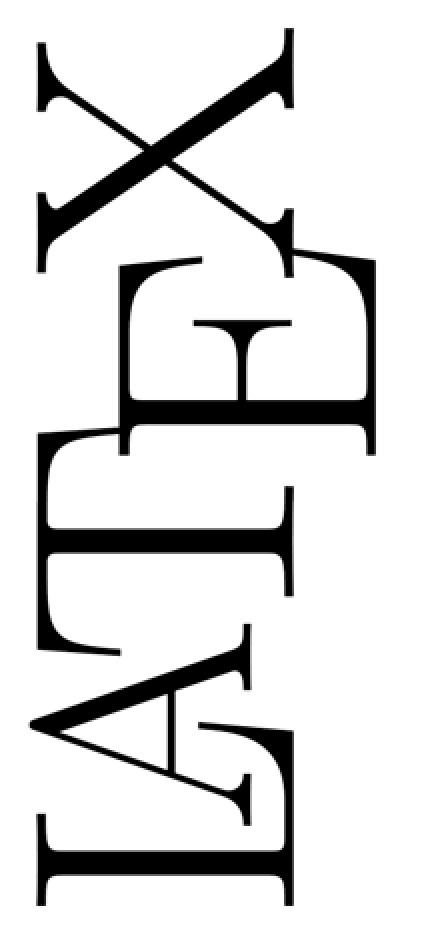
\includegraphics[scale=0.27]{latex}
  }
  \caption{Три типа представления токенов в модели BERT}\label{fig:Transformer5-BERTTokenTypes}
\end{figure}
Модель BERT предобучалась на 2 наборах данных. Это набор данных BooksCorpus, имеющий 800 миллионов слов \cite{zhu_2015}, и набор данных из английской Википедии, содержащей 2.5 миллиардов слов \cite{devlin_2018}. 

Дообучение модели BERT может производиться на любых, даже небольших наборах данных. Как и при решении задачи Next Sentence Prediction, в задачах классификации и регрессии ответ модели предсказывается линейным слоем по финальному векторному представлению [CLS] токена. В оригинальной статье показаны результаты модели BERT при дообучении на задачах из набора данных GLUE; цифры из данной статьи будут также использоваться в последующих разделах. 
Две основных конфигурации модели BERT, предложенные авторами оригинальной статьи - это:
\begin{itemize}
\item[*] BERT-BASE. Размерность векторного представления токена 768, 12 последовательно повторяющихся слоев Трансформер, 12 модулей self-attention в одном блоке, 110 миллионов параметров. Для обучения использовались 4 Cloud TPU 4 дня. 
\item[*] BERT-LARGE. Размерность векторного представления токена 1024, 24 последовательно повторяющихся слоя Трансформер, 16 модулей self-attention в одном блоке, 340 миллионов параметров. Для обучения использовалось 16 Cloud TPU 4 дня. 
\end{itemize}

Универсальность архитектуры BERT обуславливает возможность применения данной нейросетевой модели для решения широкого круга задач. Так, токен [SEP] позволяет ставить границы между поступающими на вход последовательностями. Это даёт возможность решать задачи классификации пар предложений и задачи ответа на вопрос (question answering), где тоже на вход подаются пары последовательности. Токен [MLM] даёт возможность для обучения векторных представлений токенов, зависящих от контекста, что позволяет решать также задачи классификации каждого токена в последовательности (распознавание именованных сущностей, классификация каждого слова по частям речи). Токен [CLS] содержит информацию обо всей последовательности, что даёт возможность применять его для решения задач классификации текста. 

Эффективность модели BERT обусловлена переносом знаний: BERT получает знания на этапе предобучения, и применяет их на этапе дообучения для решения иных задач. Таким образом, в модели BERT происходит перенос знаний. 

На момент проведения описанных в данной работе исследований, модель BERT(с определёнными модификациями) считалась стандартом в машинном обучении. В связи с этим, именно модели такого типа считались базовыми в дальнейшей работе, и при работе над многозадачными моделями приоритет в рассмотрении отдавался именно архитектурам, основанным на модели BERT. Применявшиеся в данной работе архитектуры многозадачных моделей будут подробнее рассмотрены ниже. 
